%%%%%%%%%%%%%%%%%%%%%%%%%%%%%%%%%%%%%%%%%%%%%%%%%%%%%%%%%%%%%%
\section{Apresentação ao Curso de PICAT}

%%%The \pause command internally uses \onslide (see §9.1 of the beamer manual), so it does employ overlay specifications.

%%%%%%%%%%%%%%%%%%%%%%%%%%
\begin{frame}[fragile]
\frametitle{Apresentação ao Curso de PICAT}
\begin{minipage}{0.47\textwidth}
    \begin{itemize}
        \item A linguagem PICAT   
        \item Requisitos e recursos
        \item O que esperar do curso?
        \item Agenda do curso
        \item Abrangência

    \end{itemize}
\end{minipage}
\begin{minipage}{0.5\textwidth}
\begin{figure}[ht!]
\begin{center}

\includegraphics[width=1.2\textwidth, height=0.40\textheight]{figures/logo_picat_alex.jpg}
\end{center}
\end{figure}
\end{minipage}

\pause
\begin{center}
\textcolor{red}{\textbf{Em resumo: Uma visão clara e precisa do que é o curso!}}
 \end{center}


\end{frame}
%%%%%%%%%%%%%%%%%%%%%%%%%%


\begin{frame}[fragile]

  \frametitle{A Linguagem PICAT}
  \begin{itemize}
    \item O que é o PICAT?
    \pause
       \begin{itemize}
			\item Uma linguagem de programação de propósitos gerais -- \textcolor{magenta}{\textbf{\textit{canivete suiço}}}
			\item Uma evolução do PROLOG (consagrada linguagem dos primórdios da IA)
			\item Tem elementos das linguagens Python, Prolog e Haskell
		\end{itemize}

    \item Uso e finalidades do PICAT:
    \pause
       \begin{itemize}
			\item Uso de programas gerais: de simples à complexos (uma reflexão)
			\item Provê suporte há vários \textit{solvers} na área de Pesquisa Operacional
			\item Área: IA, programação por restrições, programação inteira, planejamento,
			combinatória, etc
		\end{itemize}

   \end{itemize}

  \end{frame}
    
%\framebreak
\begin{frame}[fragile]
  \frametitle{Você e o Curso}
  \begin{itemize}

    \item Este curso é dirigido a você?
  \pause
    \item Requisitos:
   \pause
		\begin{itemize}
			\item Conhecimento: noções de lógica matemática 
			(proposional e primeira-ordem), matemática elementar
			e alguma outra linguagem de programação

			\item Dedicação: depende de você
			\pause
		\item \textcolor{magenta}{\textbf{Contudo: conhecimento prévio, estarei resumindo-os!}}
		\end{itemize}
		
  \pause
    \item Motivação:
   \pause
		\begin{itemize}
			\item Ao final você vai estar apto a resolver problemas
			computacionais difíceis: os famosos NP-completo!
			
			\item Difícil: muitas linhas de código e muito conhecimento de algoritmos seriam
			necessários
			
			\item Com Picat, há sofisticados esquemas prontos para se construir programas.

		\end{itemize}

  \end{itemize}

\end{frame}


    
\begin{frame}[fragile]
  \frametitle{Recursos}
  \begin{itemize}
						
    \item Recursos computacionais:\\
    \pause 
    Binários disponíveis para Linux, Mac e Windows
     e Código fonte (em C) também disponível

    \item Comunidade e ações: \url{http://picat-lang.org}
    
    \pause
    \item O material \textcolor{magenta}{\textbf{sempre}} atualizado 

    \pause
    \begin{itemize}
      \item  \textcolor{magenta}{O material do curso \textbf{completo} (e \textbf{atualizado}) em PDF,
      aqui na plataforma, junto ao material para download da $1a.$ aula}
      
     \item   Os códigos \textcolor{magenta}{fontes dos programas}:  \url{http://github.com/claudiosa/CCS/picat}
    \end{itemize}

			\item Além do material aqui disponível em PDF, o mais importante  do curso
			 vai estar na interatividade
			da minha \textcolor{magenta}{\textbf{apresentação oral}} 
			
    
  \end{itemize}

\end{frame}


\begin{frame}
\frametitle{Livro Disponível}

\begin{figure}[ht!]
\begin{center}
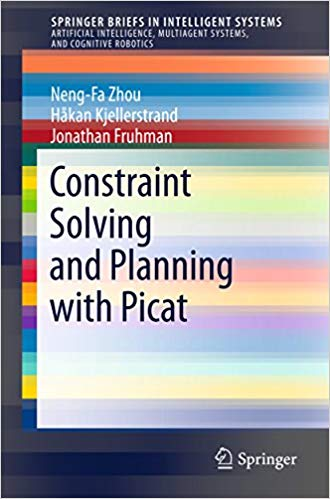
\includegraphics[width=0.5\textwidth, height=0.70\textheight]{figures/livro_picat.jpg}
\caption{Em \url{http://picat-lang.org} -- clique sobre o livro}
\end{center}
\end{figure}


\end{frame}





    
\begin{frame}[fragile]
  \frametitle{Aulas: captura de telas (\textit{screencast})}
  \begin{itemize}

    \item Há alguns pontos do curso que estão repetidos: \textit{propositalmente}!\\
    \pause
    Reforça os erros que cometi um dia!

    \pause
    \item As aulas aqui apresentadas \textbf{não} serão regravadas!
        
    \pause 
    \item Para compensar este detalhe, vamos o texto completo em PDF e fontes dos programas sempre atualizados,
    e eventuais \textcolor{red}{\textbf{vídeos-extras}} afim de  elucidar os pontos aqui abordados e/ou perguntas
    
%    \pause 
%    \item Na parte teórica da definição do Picat, mantive os padrões 
%    descritos no manual da linguagem (\url{http://picat-lang.org}).
    
  \end{itemize}

\end{frame}

    
\begin{frame}[fragile]
  \frametitle{Amostras no YouTube}
  
  \begin{itemize}

    \item Além desta  apresentação do curso, você pode assistir uma \textit{amostra}
     deste curso em aulas  que fiz no YouTube, há alguns anos atrás:

    \pause
    \item \textcolor{magenta}{\textbf{Videoaula 01: Introdução ao PICAT}}\\
    \textbf{\url {https://www.youtube.com/watch?v=0DmTyFFQPK8}}

    \pause 
    \item \textcolor{magenta}{\textbf{Videoaula 02: Tipos de Dados do PICAT}}\\
    \textbf{\url {https://www.youtube.com/watch?v=7fPKPd0ZDnc}} 
    
    \item Estas aulas são introdutórias e o curso vai muito mais além destes
    assuntos.
    
    \pause 
    \item Estas videoaulas foram refeitas e  encontram-se com uma nova abordagem
    neste curso. 
    
  \end{itemize}

\end{frame}




\begin{frame}[fragile]
  \frametitle{Ao Final do Curso}
  \begin{itemize}

						
    \item Terás uma sólida visão  de uma linguagem
    utilizada em várias áreas tais como: modelagem matemática, IA,
    Pesquisa Operacional, etc

    \pause
    \item Vais conseguir resolver problemas com alguma complexidade e ler
    códigos de grandes programadores da área: Barták, Neng-Fa, Hakank, Dymichenko, etc    
    
    \pause
		\item Em resumo, este material é  um guia para o seu desenvolvimento,
		 com explicações nestas aulas, que funcionam como um \textcolor{magenta}{\textbf{\textit{atalho}}}
		  de horas de estudo sobre vários temas apresentados.
   
    \pause
    \item A seguir os temas cobertos no curso com PICAT:
  \end{itemize}

\end{frame}




\subsection{Conteúdo do Curso}
			
\begin{frame}[fragile]
  \frametitle{Conteúdo}
  \begin{enumerate}

					
    \item  \underline{Introdução} ($\approx$ 27 min):\\
    Histórico, paradigmas de linguagens, usando o Picat, etc

    \pause
    \item \underline{Tipos de Dados e Variáveis} ($\approx$ 28 min):\\
Tipos de Dados, Variáveis, Unificação e Atribuição, Tabela de Operadores, Operadores Especiais,
 Exemplos
    
    \pause
		\item \underline{Predicados e Funções} ($\approx$ 32 min):\\
Casamento de padrões, funções, regras, fatos, metas, exemplos
		
    \pause
    \item \underline{Estruturas de Decisão, Laços e Iteradores} ($\approx$ 28 min):\\
Estruturas de decisão, iteradores, funções e predicados especiais, 
entradas e saídas, exemplos
    
    \pause
		\item  \underline{Recursão} ($\approx$ 28 min):\\
     Conceitos de recursão, conceito de \textit{backtracking}, o paradigma
     de pensar e programar recursivamente, exemplos
\end{enumerate}

\end{frame}




			
\begin{frame}[fragile]
  \frametitle{Conteúdo}
  
  \begin{enumerate}

   \setcounter{enumi}{5}
    \item  \underline{Listas} ($\approx$ 36 min):\\
    Definição, como o Picat opera as listas, exemplos


    \pause
    \item  \underline{Buscas} ($\approx$ 40 min):\\
    Definições, uso, abrangência, exemplos

    \pause
    \item \underline{Programação Dinâmica (PD)} ($\approx$ 24 min):\\
        Definições, uso, abrangência, exemplos

    
    \pause
    \item \underline{Planejamento} ($\approx$ 35 min):\\
        Definições, o módulo \textit{planner}, uso, abrangência, exemplos

    \pause
		\item \underline{Programação por Restrições (PR)} ($\approx$ 85 min):\\
      Definições, o módulo \textit{cp}, uso, abrangência, exemplos (03).
      Técnicas de PR.\\
      3 aulas aqui: $1a.$ aula $\approx$ 41 min, $2a.$ aula $\approx$ 16 min,
      $3a.$ aula $\approx$ 28 min
      
    
\end{enumerate}

\end{frame}


			
\begin{frame}[fragile]
  \frametitle{Conteúdo}
  
  \begin{enumerate}

   \setcounter{enumi}{10}

		\item  \underline{Conclusões} ($\approx$ 9 min):\\
    Retrospectiva, tendências, o que ficou faltando, dicas de programação, etc

    \pause
		\item  \underline{Exercícios}: \\
    Uma lista de exercícios sobre Picat será disponibilizado aqui na Plataforma

    
\end{enumerate}

\end{frame}


\subsection{Agradecimentos}

  %%%%%%%%%%%%%%%%%%%%%%%%%%%%%%%%%%%%%%%%%%%%%%%%%%%%%%%%%%%%%%%%%%%%%
\begin{frame}[fragile]
  \frametitle{Contribuições e Agradecimentos}

  \begin{itemize}
  \item Miguel Alfredo Nunes
  \item Jeferson L. R. Souza
    \item Alexandre Gonçalves 
    \item Hakan Kjellerstrand -- (\url{http://www.hakank.org/picat/})
    \item Neng-Fa Zhou -- (\url{http://www.picat-lang.org/})
    \item João Herique Faes Battisti
    \item Paulo Victor de Aguiar
    \item Rogério Eduardo da Silva
    \item Outros anônimos que auxiliaram na produção deste documento
    \item Tem muita gente aqui ... enumerá-los posso ser injusto com alguém!
  \end{itemize}

\end{frame}


\begin{frame}[fragile]
  \frametitle{Obrigado ...}

\begin{minipage}{0.47\textwidth}
\begin{Large}
\begin{center}
\textbf{\textcolor{magenta}{... e vejo vocês\\ no curso!}}
\end{center}
\end{Large}
\end{minipage}
\begin{minipage}{0.5\textwidth}
\begin{figure}[ht!]
\begin{center}

\includegraphics[width=1.2\textwidth, height=0.40\textheight]{figures/logo_picat_alex.jpg}
\end{center}
\end{figure}
\end{minipage}



\end{frame}
						
